\documentclass{beamer}
%% apparently this magic helps avoid the dreaded
%% ``Too many math alphabets used in version normal''
%% error. Yuk.
\newcommand\hmmax{0}
\newcommand\bmmax{0}
%% end magic

\usepackage{amssymb,amsmath,amsthm}
\usepackage{latexsym}

\usepackage{array}

\usepackage{url}
\usepackage{hyperref}

%% uses the AMS Euler math font.
\usepackage{euler}

%% for coloneqq
%% \usepackage{mathtools}

%% for \underaccent
\usepackage{accents}

% for semantic brackets
%% \usepackage{stmaryrd}

% for inference rules
\usepackage{proof}

%% for mathpar environment
\usepackage{mathpartir}

% for \scalebox, \rotatebox
%% \usepackage{graphicx}

%% for colors
\usepackage{color}

%% for drawing Hasse diagram
\usepackage{tikz}

%% for censoring things
\usepackage{censor}


%% Commands
\newcommand{\mto}{\overset{\textbf{+}\:}{\to}}
\newcommand{\eq}[1]{\underaccent{\mathit{eq}}{#1}}
\newcommand{\fin}[1]{\underaccent{\mathit{fin}}{#1}}
\newcommand{\m}[1]{\ensuremath{\mathbf{#1}}}
\newcommand{\ms}{\mathsf}
\newcommand{\N}{\mathbb{N}}
\newcommand{\x}{\times}


%% Metadata
\title{Datafun}
\author{Michael Arntzenius\inst{1} \and Neel Krishnaswami\inst{2}}
\institute{\inst{1}University of Birmingham \and \inst{2}University of Cambridge}
\date{ICFP 2016}

\begin{document}

\maketitle


\begin{frame}
  \Large
  \begin{tabular}{rl}
    1 & \texttt{\censor{x := 0}}\\
    2 & \texttt{\censor{t := 3}}\\
    3 & \texttt{\censor{while true do}}\\
    4 & \texttt{\quad \censor{s := if x = 0}}\\
      & \texttt{\quad \phantom{s := }\censor{then 7}}\\
      & \texttt{\quad \phantom{s := }\censor{else 4 + t}}\\
    5 & \texttt{\quad \censor{x $\leftarrow$ x + 1}}\\
    6 & \texttt{\quad print s}
        \qquad \texttt{\#} can be replaced by \texttt{print 7}
  \end{tabular}
\end{frame}

\begin{frame}
  \Large
  \begin{tabular}{rl>{\hspace{1em}}l}
    1 & \texttt{x := 0} & x = 0\\
    2 & \texttt{\alt<2->{t := 3}{\censor{t := 3}}}
      & \uncover<2->{x = 0, t = 3}\\
    3 & \texttt{\alt<3->{while true do}{\censor{while true do}}}
      & \uncover<3->{x = 0, t = 3}\\
    4 & \texttt{\quad \alt<4->{s := if x = 0}
                              {\censor{s := if x = 0}}}
      \\
      & \tt \quad \phantom{s :=} \alt<4->{then 7}{\censor{then 7}}
      & \uncover<4->{x = 0, t = 3, s = \alt<5->{7}{\color{red}{?}}}\\
      & \texttt{\quad \phantom{s := }\alt<4->{else 4 + t}{\censor{else 4 + t}}}\\
    5 & \texttt{\quad \alt<6->{x $\leftarrow$ x + 1}
                              {\censor{x $\leftarrow$ x + 1}}}
      & \uncover<6->{x = 1, t = 3, s = 7}\\
    6 & \texttt{\quad print s}
      & \uncover<7->{x = 1, t = 3, s = 7}
  \end{tabular}
\end{frame}

\begin{frame}
  \Large
  \begin{tabular}{rl>{\hspace{1em}}l}
    1 & \texttt{x := 0} & x = 0\\
    2 & \texttt{t := 3} & x = 0, t = 3\\
    \color<1,7>{red}
    3 & \texttt{\color<1,7>{red} while true do}
      & {\color<1,7>{red} x = $\top$, t = 3}\\
    \color<1>{gray}\color<2-4>{red}
    4 & \color<1>{gray}\color<2-4>{red}
        \tt\quad s := if x = 0\\
      & \color<1>{gray}\color<2-4>{red} \tt\quad\phantom{s :=} then 7
      & \color<1>{gray}\color<2-4>{red}
        x = \alt<3->{$\top$}{{\color<2>{gray}0}}, t = 3, s = {\color<2-3>{gray}7}\\
      & \color<1>{gray}\color<2-4>{red}
        \tt\quad\phantom{s :=} else 4 + t\\
    \color<1-4>{gray}\color<5>{red}
    5 & \color<1-4>{gray}\color<5>{red}
        \texttt{\quad x $\leftarrow$ x + 1}
      & \color<1-4>{gray}\color<5>{red}
        x = \alt<5->{$\top$}{1}, t = 3, s = 7\\
    \color<1-5>{gray}\color<6>{red}\color<8>{blue}
    6 & \color<1-5>{gray}\color<6>{red}\color<8>{blue} \texttt{\quad print s}
      & \color<1-5>{gray}\color<6>{red}
        x = \alt<6->{$\top$}{1}, t = 3, {\color<8>{blue} s = 7}
  \end{tabular}
\end{frame}


\begin{frame}
  \Large Computing \textbf{fixed points}\\of \textbf{monotone maps}\\on
  \textbf{semilattices}\\ satisfying an \textbf{ascending chain condition}
\end{frame}


\begin{frame}
  %% {\footnotesize\color{gray} Datafun is a \emph{pure}, \emph{total} functional
  %%   language for expressing \textbf{\color{black} fixed points} of
  %%   \textbf{\color{black} monotone maps} on \textbf{\color{black} semilattices}
  %%   satisfying an \textbf{\color{black} ascending chain condition}.}

  %% \vspace{0.5em}

  \large
  \begin{itemize}
  \item \textbf{Fixed point}: Keep going until nothing changes.
    %% FIXME: increasing vs monotone
  \item \textbf{Monotone}: Unidirectional: $\bot \Rightarrow \text{constant} \Rightarrow \top$
  \item \textbf{Semilattice}:\\

    \begin{center}\large
      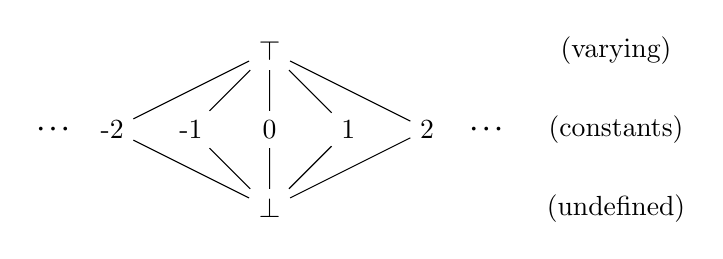
\begin{tikzpicture}[scale=1]
        \node (top)  at ( 0, 1) {$\top$};
        \node (bot)  at ( 0,-1) {$\bot$};
        \node (-3)   at (-2.75, 0) {$\hdots$};
        \node (-2)   at (-2, 0) {-2};
        \node (-1)   at (-1, 0) {-1};
        \node (0)    at ( 0, 0) {0};
        \node (1)    at ( 1, 0) {1};
        \node (2)    at ( 2, 0) {2};
        \node (3)    at ( 2.75, 0) {$\hdots$};
        %% TODO: left-align these
        \node (varying)   at (4.4, 1) {\normalsize (varying)};
        \node (constant)  at (4.4, 0) {\normalsize (constants)};;
        \node (undefined) at (4.4,-1) {\normalsize (undefined)};
        \draw (bot) -- (-2) -- (top) -- (-1) -- (bot) -- (0) -- (top)
        -- (1) -- (bot) -- (2) -- (top);
      \end{tikzpicture}
    \end{center}

  \item \textbf{ACC}: Can't go up forever.
  \end{itemize}

\end{frame}


\begin{frame}%{What's expressible this way?}

  \large Computing \textbf{fixed points} of \textbf{monotone maps} on
  \textbf{semilattices} satisfying an \textbf{ascending chain condition}\\
  is very general:

  \Large %% {What's expressible this way?}\vspace{0.3em}
  \begin{itemize}
  \item Static analyses
  \item Graph algorithms: reachability, shortest path, ...
  \item Parsing context-free grammars
  \item Datalog {\large (as long as the semilattice is finite sets)}
  \end{itemize}

  %% Surprisingly general!
\end{frame}


\begin{frame}

  \Large \textbf{Datafun} is:
  \begin{itemize}
  \item a simply-typed lambda calculus
  \item where types are posets \& some are semilattices
  %% \item ... of which some are semilattices
  \item that \textbf{tracks monotonicity via types}
  \item to let you compute fixed points.
  \end{itemize}
\end{frame}

\begin{frame}
  %% \frametitle{How to express these fixed points?}

  %% \Large\vspace{-2em}
  %% {\huge\[ \alt<2->{\ms{fix}\;\m{x}\;\ms{is}\;[...]}
  %%   {\ms{fix}\;(\lambda \m{x}.\; [...])} \]}

  \Large\vspace{-2em}
  {\huge\[ {\ms{fix}\;(\lambda \m{x}.\; [...])} \]}

  Need to check:
  \begin{enumerate}
  \item $(\lambda \m{x}.\; [...])$ is \textbf{monotone}
    \qquad \color[rgb]{0.5,0,1.0} $\leftarrow$ \emph{novel?}
  \item \color{gray} on a \textbf{semilattice} 
  \item satisfying \textbf{ACC}.
  \end{enumerate}

  %% NOTE: mention that monotonicity is NOVEL.

\end{frame}

%% \begin{frame}
%%   \begin{center}
%%     \huge\bf Track monotonicity with types!
%%   \end{center}
%% \end{frame}

\begin{frame}
  \frametitle{Types as posets}
  \large
  \begin{center}
    \begin{tabular}{cll}
      \textbf{Type} & \textbf{Meaning} & \textbf{Ordering}
      \\\hline
      $\mathbb{N}$ & naturals & $0 < 1 < 2 < \hdots$\\
      $2$ & booleans & $\ms{false} < \ms{true}$\\
      $\{A\}$      & finite sets & ${\subseteq}$\\
      $A \times B$ & pairs & pointwise\\
      %% $\ms{Flat}\;A$ &
      %% %% an $A$ or $\bot$ or $\top$ &
      %% \multicolumn{2}{m{4cm}}{\scriptsize
      %%   \begin{tikzpicture}[scale=0.5]
      %%   \node (top)  at ( 0, 1) {$\top$};
      %%   \node (bot)  at ( 0,-1) {$\bot$};
      %%   \node (-2)   at (-1.49, 0) {$\hdots$};
      %%   \node (-1)   at (-0.75, 0) {$\hdots$};
      %%   \node (0)    at ( 0, 0) {$A$};
      %%   \node (1)    at (0.75, 0) {$\hdots$};
      %%   \node (2)    at (1.49, 0) {$\hdots$};
      %%   \draw (bot) -- (-2) -- (top) -- (-1) -- (bot) -- (0) --
      %%         (top) -- (1) -- (bot) -- (2) -- (top);
      %% \end{tikzpicture}}\\
      $A \to B$    & functions & pointwise\\
      $A \mto B$  & \textbf{monotone} functions & pointwise\\
    \end{tabular}
  \end{center}

  \vspace{0.75em}\pause

  \[\begin{array}{l}
    member ~:~ \mathbb{N} \to \{\mathbb{N}\} \mto 2\\
    member\; x\; \mathbf{s} = \exists(y \in \mathbf{s})\; x = y
  \end{array}\]

  \vspace{5em}

\end{frame}

%% monotone vs discrete
%% example: set membership
\begin{frame}
  \frametitle{Tracking monotonicity}

  %% Comment this list out and just speak it?
  \Large
  \begin{itemize}
  \item Two types of \emph{function}: discrete or monotone
  \item Two kinds of \emph{variable}: discrete or monotone
  \item Two \emph{typing contexts}: $\Delta$ discrete, $\Gamma$ monotone
  \end{itemize}

  {\huge\[\Delta;\Gamma \vdash e : A\]}

  \begin{quote}
    \hspace{-1.1ex}``$e$ has type $A$ with free variables $\Delta,\Gamma$;\\
    moreover, $e$ is monotone in $\Gamma$.''
  \end{quote}
\end{frame}


%% ---------- TYPING RULES ----------
\begin{frame}{Function application}
  %% \frametitle{Typing rules: discrete vs monotone}
  \Large

  \begin{mathpar}
    \infer[\textsc{\normalsize monotone app}]
          {\Delta;\Gamma \vdash f\, a : B}
          { \Delta;\Gamma \vdash f : A \mto B \hspace{1em}&
            {\color<2->{red}\Delta;\Gamma} \vdash a : A }
    \pause\vspace{0.5em}

    \infer[\textsc{\normalsize discrete app}]
          {\Delta;\Gamma \vdash f\, a : B}
          { \Delta;\Gamma \vdash f : A \to B \hspace{1em}&
            {\color{red}\Delta;\emptyset} \vdash a : A }
  \end{mathpar}

  \pause\vspace{0.5em}

  Otherwise:
  \[\begin{array}{l}
  coerce ~:~ (\mathbb{N} \to \mathbb{N}) \to (\mathbb{N} \mto \mathbb{N})\\
  coerce\; f\; \mathbf{x} = f\; {\color{red}\mathbf{x}}
  \end{array}\]
\end{frame}

\begin{frame}{Finite sets}\Large
  \[
  \begin{array}{rcl}
    e &::=& ... ~|~ \{\} ~|~ e \cup e ~|~ \{e\} ~|~ \bigcup(x \in e)\, e\\
      \pause&~|~& \{e ~|~ x \in e, ...\}
  \end{array}
  \]

  \pause

  \begin{mathpar}
    \infer{\Delta;\Gamma \vdash \{e\} : \{A\}}{\Delta;{\color{red}\emptyset} \vdash e : A}
    %% \and\pause\color{gray}
    %% \infer{\Delta;\Gamma \vdash \{\} : \{A\}}{}
    %% \and
    %% \infer{\Delta;\Gamma \vdash e_1 \cup e_2 : \{A\}}{\Delta;\Gamma \vdash e_i : \{A\}}
    %% \and
    %% \infer{\Delta; \Gamma \vdash \bigcup(x \in e_1)\ e_2 : \{B\}}{
    %%   \Delta;\Gamma \vdash e_1 : \{A\} \quad&
    %%   \Delta,x\!:\!A; \Gamma \vdash e_2 : \{B\}
    %%   }
  \end{mathpar}
\end{frame}


\begin{frame}{{\it Example:} Relational composition}\Large
  \[\begin{array}{l}
    (\bullet) : \{A \times \eq{B}\} \mto \{\eq{B} \times C\} \mto \{A \times C\}\\
    \m{s} \bullet \m{t} =
    \{(x,z) ~|~ (x,y) \in \m{s}, (!y,z) \in \m{t}\}
  \end{array}\]
\end{frame}

\begin{frame}{{\it Example:} Reachability}\Large
  \[\begin{array}{l}
    path ~:~ \{\fin{A} \times \fin{A}\} \mto \{\fin{A} \times \fin{A}\}\\
    path\;\m{E} = \ms{fix}~\m{P}~\ms{is}~ \m{E} \cup (\m{P} \bullet \m{P})
  \end{array}\]

  \vspace{1.5em}

  In Datalog:\vspace{1em}\\
  \begin{tabular}{l}
    \texttt{path(X,Y) :- edge(X,Y).}\\
    \texttt{path(X,Z) :- path(X,Y), path(Y,Z).}\\
  \end{tabular}
\end{frame}


%% Parsing.
\begin{frame}{{\it Example:} CYK Parsing}
  \large

  Nonterminals: $A, B, C...$\\
  Literal strings: ${s}, {t}, ...$\vspace{1em}\\
  Rules are all of the form $A \to B\,C$ or $A \to {s}$.\pause
  \vspace{1em}\\

  Apply the following inference rules \textbf{to saturation}:\pause
  \vspace{0.5em}
  \Large\begin{mathpar}
    \infer{A(i,j)}{A \to {s} & w[i..j] = {s}}
    \and
    \infer{A(i,k)}{A \to B\,C & B(i,j) & C(j,k)}
  \end{mathpar}

  \vspace{0.5em}\large

  where $A(i,j) =$ ``$A$ produces the substring $w[i..j]$''\\
  and $w$ is the input string
\end{frame}

\begin{frame}{{\it Example:} CYK Parsing}
  \[\begin{array}{l}
    \textbf{type}~\ms{rule} = \textsc{Concat}(\ms{symbol}, \ms{symbol})
    ~|~ \textsc{String}(\ms{string})\\
    \textbf{type}~\ms{grammar} = \{\ms{symbol} \times \ms{rule}\}\\
    \textbf{type}~\ms{fact} = \ms{symbol} \x \N \x \N\\
    \\
    \ms{step} ~:~ \ms{string} \to \ms{grammar} \to \{\ms{fact}\} \mto \{\ms{fact}\}\\
    \ms{step}\; w\; G\; \m{prev} =\\
    \quad \phantom{\cup}~\{ (a,i,k) ~|~ (a, \textsc{Concat}(b,c)) \in G,\\
    \quad \phantom{\cup}~\hspace{4.24em} (!b,i,j) \in \m{prev},
                   (!c,!j,k) \in \m{prev} \}\\
    \quad\cup~ \{ \, (a, i, i + \ms{length}\;s)\\
    \quad\phantom{\cup}\,~|~ (a, \textsc{String}(s)) \in G,\\
    \quad\phantom{\cup\,~|~} i \in \ms{range}\; 0\; (\ms{length}\; w - \ms{length}\; s),\\
    \quad\phantom{\cup\,~|~} s = \ms{substring}\; w\; i\; (i + \ms{length}\; s) \}
  \end{array}\]
\end{frame}

%% \begin{frame}{Example: reaching definitions}
%%   %% TODO: try to make this more legible (larger)
%%   \vspace{-4em}
%%   \[\begin{array}{l}
%%     \textsf{// omitted for brevity}\\
%%     \textbf{type}~\ms{stmt}, \ms{line}, \ms{var}\\
%%     \ms{defines} ~:~ \ms{stmt} \to \{\ms{var}\}\\
%%     \\
%%     \ms{reachingDefs} ~:~ \{\ms{line} \x \ms{stmt}\} \to \{\ms{stmt} \x \ms{stmt}\}
%%     \to \{\ms{line} \x \ms{line} \x \ms{var}\}\\
%%     \ms{reachingDefs}\, code\, flow =\\
%%     \quad \ms{fix}~\m{self}~\ms{is}\\
%%     \quad\quad \bigcup ((i,s) \in code)\\
%%     \quad\quad\quad \phantom{\cup~} \{(i,i,v) ~|~ v \in \ms{defines}\,s\}\\
%%     \quad\quad\quad \cup~ \{(i,l,v) ~|~ (j, !i) \in flow, (!j,l,v) \in \m{self},
%%     \neg (v \mathrel{{\in}?} \ms{defines}\,s)\}\\
%%   \end{array}\]
%% \end{frame}

%% More examples?

%% val subsets: {nat} →⁺ {{nat}}
%% fun subsets univ =
%%   fix s = {{}}
%%         ∨ {{x} | x in univ}
%%         ∨ {x ∨ y | x in s, y in s}

%% val rd : code -> flow -> {label, label, var}
%% fun rd code flow =
%%   fix self = for ((i,s) ∈ entries code)
%%                {(i, i, v) | v ∈ defines s}
%%              ∨ {(i, l, v) | (j, .i) ∈ flow, (.j, l, v) ∈ self
%%                           , not (v ∈? defines s)}


\begin{frame}{Summary}\large

  \begin{itemize}
  \item Many algorithms are concisely expressed as \textbf{fixed points} of
    \textbf{monotone maps} on \textbf{semilattices}.
  \item Datafun is a simple, pure, and total language for computing these fixed
    points.
  \item Key idea: \textbf{track monotonicity with types}!
    %% something about ACC
  \item In effect, generalizes Datalog to other semilattices.
  %% \item plus, we get functional abstraction!
  \end{itemize}

  \vspace{1em}
  \begin{center}
    {\Large \url{github.com/rntz/datafun}}
  \end{center}
\end{frame}


%% Post-presentation matter
\begin{frame}
  \centering \Huge \textsc{Fin.}
\end{frame}

\begin{frame}{Future work}\large
  \begin{itemize}
  \item Optimization
    \begin{itemize}\normalsize
    \item Semi-na\"ive evaluation
    \item Dataflow (push \& pull)
    \item Magic sets
    \end{itemize}
  \item More semilattice types
  \item More flexible termination/ACC checking
  \item Aggregation operations (summing, averaging)
    \begin{itemize}\normalsize
    \item Commutative monoids?
    \end{itemize}
  \item Other applications of types for monotonicity
    \begin{itemize}\normalsize
    \item Types for functoriality?
    \item LVars \& monotone processes
    \end{itemize}
  \end{itemize}
\end{frame}

\begin{frame}
  \frametitle{Datafun vs Datalog}

  \begin{center}
    \begin{tabular}{l|l}
      \textbf{Datafun pros} & \textbf{Datalog pros}\\\hline
      Functional abstraction! & Finiteness/ACC is automatic\\
      Semilattices other than $\mathcal{P}_{\ms{fin}}$ & Often more concise\\
      Can do arithmetic & Existing optimization literature\\
      Can nest sets
    \end{tabular}
  \end{center}

  \vspace{2em}

  \textbf{See also}: \textsc{Flix}, PLDI 2016, Madsen et al
\end{frame}

\begin{frame}
  \frametitle{Datafun vs \textsc{Flix}}

  \begin{center}
    \begin{tabular}{l|l}
      \textbf{Datafun pros} & \textsc{Flix}\textbf{ pros}\\\hline
      Functions on relations & Programmer-defined semilattices\\
      Types for monotonicity & No types for monotonicity
    \end{tabular}
  \end{center}
\end{frame}

\begin{frame}{Boolean elimination in a monotone world}\large

  \begin{mathpar}
    \infer[\textsc{Discrete If}]
          {\Delta;\Gamma \vdash \ms{if}~e_1~\ms{then}~e_2~\ms{else}~e_3 : A}
          { \Delta;{\color{red}\emptyset} \vdash e_1 : 2
          \quad& \Delta;\Gamma \vdash e_2 : A
          \quad& \Delta;\Gamma \vdash e_3 : A}
    \vspace{1em}\and
    \infer[\textsc{Monotone If}]
          {\Delta;\Gamma \vdash \ms{if}~e_1~\ms{then}~e_2~\ms{else}~\varepsilon : L}
          { \Delta;\Gamma \vdash e_1 : 2
          \quad
          & \Delta;\Gamma \vdash e_2 : L}
  \end{mathpar}

  \vspace{0.5em}

  For example:\vspace{-0.5em}
  \[\begin{array}{l}
    \ms{guard} ~:~ 2 \mto \{A\} \mto \{A\}\\
    \ms{guard}\; \m{c}\; \m{s} = \ms{if}~\m{c}~\ms{then}~\m{s}~\ms{else}~\{\}
  \end{array}\]
\end{frame}

\end{document}
